\begin{frame}
  \begin{center}
    {\bf Pretty Good Privacy / Gnu Privacy Guard}
  \end{center}
\end{frame}

\begin{frame}
  \frametitle{Pretty Good Privacy / Gnu Privacy Guard}
  \begin{itemize}
    \item PGP was Invented By Phil Zimmermann in 1991,
    \item Hybrid Cipher: asymmetric encryption with symmetric encryption,
    \item allows to sign communications and files for authentication,
    \item very low vulnerability count over the years~\footnote{https://cve.circl.lu/search/gnupg/gnupg},
    \item One can generate collisions on short IDs though\footnote{\url{https://github.com/lachesis/scallion/}},
    \item no Perfect Forward Secrecy,
    \item but sessions keys.
  \end{itemize}
\end{frame}

\begin{frame}
  \frametitle{Pretty Good Privacy / Gnu Privacy Guard}
            \begin{figure}[h!]
              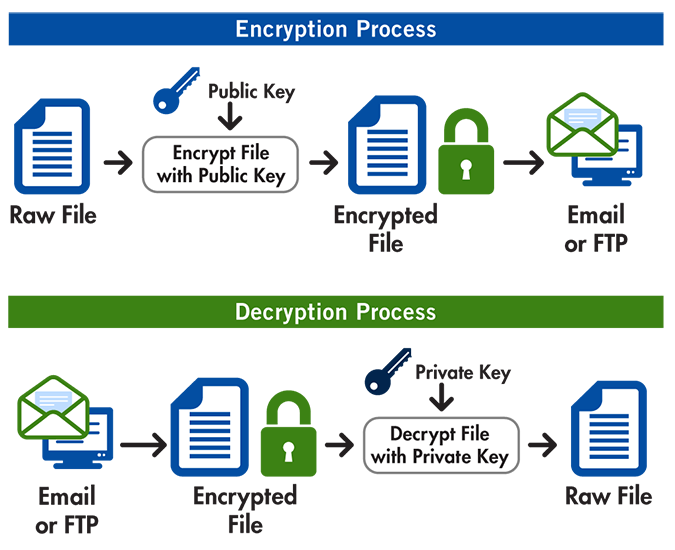
\includegraphics[width=250pt]{./gpg.png}
            \end{figure}
\end{frame}

\begin{frame}
  \frametitle{Pretty Good Privacy / Gnu Privacy Guard}
            \begin{figure}[h!]
              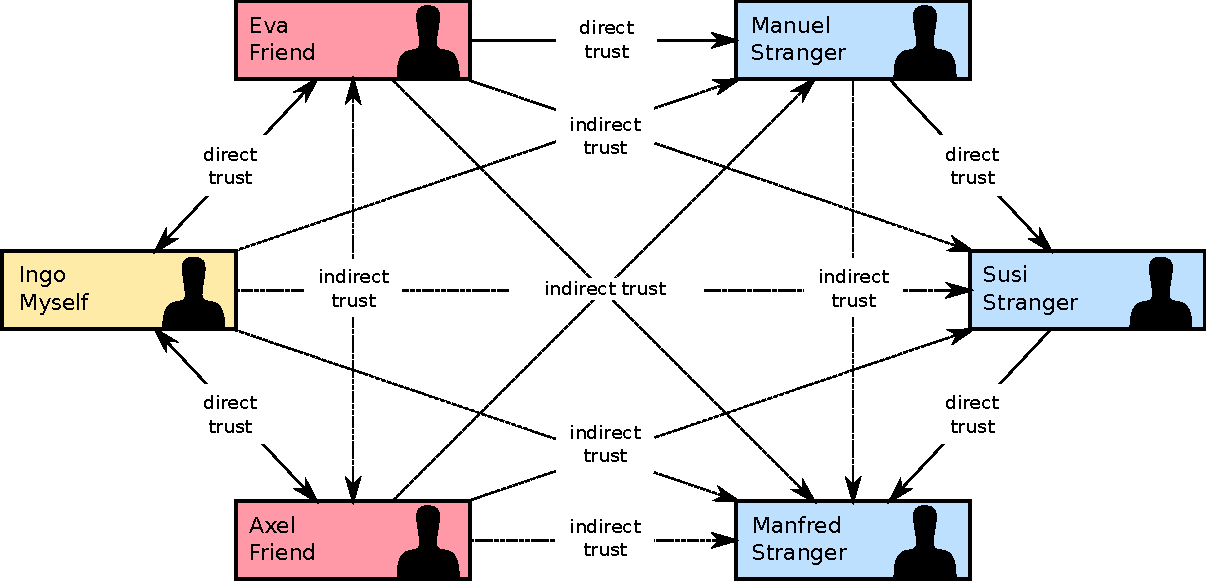
\includegraphics[width=300pt]{./wot.pdf}
            \end{figure}
\end{frame}

\begin{frame}[fragile]
  \frametitle{Gnu Privacy Guard: Session keys}

  \begin{itemize}
    \item {\bf Hands-on}
  \begin{lstlisting}
  Move into ~/hands-on/GPGsessions
  \end{lstlisting}
    \item We create two keys, one for the person being the focused of an
      investigation A (The Very Bad Guy), and one for a witness B (Mr. Good Guy),
    \item then, we encrypt two messages:
      \begin{itemize}
       \item one from A to B: to\_encrypt\_relevant.asc,
       \item and a note, form B to B (note): to\_encrypt\_irrelevant.asc, 
      \end{itemize}
    \item B's passphrase is ``goodguypassphrase'',
    \item act as B and extract the session key for to\_encrypt\_relevant.asc,
    \item act as a cop and use the session key to decrypt
      to\_encrpyt\_relevant.asc,
    \item verifies that it does not work to decrypt to\_encrypt\_irrelevant.asc.
  \end{itemize}
\end{frame}
